\chapter{Fringing Effects in MIRI}\label{ch:fringe}
Understanding optical and instrumental effects is critical for creating accurate simulated observations and for characterizing systematics. 
These systematics and uncertainties in turn impact the potential science results from any instrument by biasing measurements, reducing the signal to noise ratio of measurements or by injecting non-physical signals and correlations.
The aim of this chapter is to examine fringing in the MIRI detectors and how this effect is modeled in the instrumental simulator (MIRISIM). 

\section{Fringing}
Thin film interference occurs when light is coherently reflected at the boundary between two layers and interferes with the incident light.
This is the principle on which Fabry-P\'{e}rot interferometers function.
As we wish to determine the effect of fringing on the amplitude of the signal received by the detector, we are effectively interested in the transmittance of a series of Fabry--P\'{e}rot interferometers. 
Assuming an ideal plane-parallel optical cavity with a reflectance R at both boundaries, thickness D, and an angle $\theta$ at which the light travels within the cavity, we can compute the transmittance as:
\begin{equation}\label{eqn:trans}
T_{c} = \frac{1}{1+\frac{4R}{\left(1-R\right)^{2}}\sin^{2}\left(\frac{\delta}{2}\right)}
\end{equation}
Where the phase $\delta$ at half a wavelength ($\phi = \pi$), with wavenumber $\sigma$ is:
\begin{equation}\label{eqn:phase}
\delta = 4\pi\sigma D \cos\theta - (\phi - \pi)
\end{equation}
Systems with a spacing on the order of millimeters produces significant interference for infrared light \autocite{Lahuis2003}.

The detectors of the MRS consist of several layers, as shown in Fig. \ref{fig:layers}, with a characteristic thickness of ~500$\mu$m, which results in significant (10\%-30\%) `fringing' in a spectrally flat signal - visible in Fig. \ref{fig:flatfield}.
While this is typical for infrared detectors such as those in the Spitzer Space Telescope \autocite{Lahuis2003} or in the Space Telescope Imaging Spectrograph on board HST \autocite{Malumuth2003}, the sensitivity and spectral resolution of the MRS increase the significance of this issue.
The MIRI consortium has stated that the error budget for all detector effects must be 3.3\% or less. 
Present fringing corrections result in a 5\% deviation from a photometrically accurate signal, and can introduce correlated noise which will degrade any measured spectrum.
Therefore it is critical to examine the impact of fringing on a signal, the parameters that influence the fringing strength and phase, and possible solutions for fringe correction. 
While a more complete treatment of proposed fringe correction can be found in \autocite{Argryiou2020}, this work will examine the implementation of fringing into the MIRI instrumental simulator and address the current state of fringe correction in the JWST Data Calibration Pipeline.

\definecolor{lightgray}{HTML}{E0E0E0}
\definecolor{darkgray}{HTML}{383838}
\begin{figure}
	\centering
	\begin{scriptsize}
	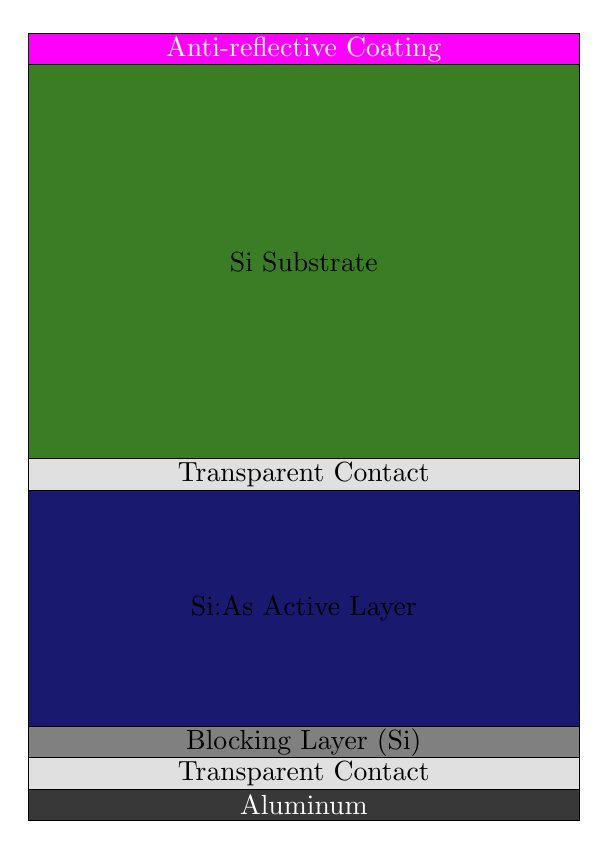
\begin{tikzpicture}
		\filldraw [fill=darkgray, draw=Black](0,0) rectangle (7,0.4) node [pos=0.5] {\textcolor{White}{Aluminum}};
		\filldraw [fill=lightgray, draw=Black](0,0.4) rectangle (7,0.8) node [pos=0.5] {Transparent Contact};
		\filldraw [fill=Gray, draw=Black](0,0.8) rectangle (7,1.2) node [pos=0.5] {Blocking Layer (Si)};
		\filldraw [fill=MidnightBlue, draw=Black](0,1.2) rectangle (7,4.2) node [pos=0.5] {Si:As Active Layer};
		\filldraw [fill=lightgray, draw=Black](0,4.2) rectangle (7,4.6) node [pos=0.5] {Transparent Contact};
		\filldraw [fill=OliveGreen, draw=Black](0,4.6) rectangle (7,9.6) node [pos=0.5] {Si Substrate};
		\filldraw [fill=Fuchsia, draw=Black](0,9.6) rectangle (7,10) node [pos=0.5] {\textcolor{White}{Anti-reflective Coating}};
	\end{tikzpicture}
	\end{scriptsize}
	\caption{Layers of the MIRI MRS detectors. Note that thicknesses are not to scale \autocite{MIRI7}.}
	\label{fig:layers}
\end{figure}

% - FRINGING REQUIREMENTS FOR MIRI - context
% - sub percent residuals - is this true and if so how much does it impact real spectral %features?
% - What has been done so far - fitting, optical modelling
% - only for some channels
% - Might remove actual spectral features as well - justification for this work (especially re posn dependence)
% - need to reproduce plots from fringing white paper
% - explain why point sources are harder (angle => optical thickness => large phase shift)
% - 
 \cite{Lahuis2018} %MIRI MRS FM Fringing Analysis
\section{MIRISIM}
\cite{Consortium2018} %Mirisim documentation
\cite{Cossou2019} %MIRISIM in python
The MIRI instrument has been modeled in python as a program known as MIRISM. 
This program takes in an astronomical 'scene' along with some configuration parameters to output a detector data product, similar to what will be produced by the actual instrument.
This is relatively full-featured simulator, modelling the instrumental PSF, various noise sources and distortion maps, among other effects.
While MIRISIM is functional for all of the MIRI sub-instruments, this report will only deal with the Medium-Resolution Spectrometer (MRS) sub instrument, described in section \ref{sec:mrs}.
The goal of this section is to describe the implementation and testing of an updated optical model of the `fringing' effect - an optical effect caused by thin film interference from the multiple layers of the detector.
\subsection{Architecture}
SCENE - SEDs
SIMULATOR
PYSPECSIM
\subsection{Data Products}
\begin{figure}
	%\includegraphics[width=\linewidth]{}
	\caption{\label{fig:fringeflat}}
\end{figure}
\subsection{Instrumental effects}
\subsection{Fringing}
\cite{Lahuis2003} %Spitzer fringes
\cite{VanderPlas2018} % Understanding lomb-scargle - identifing periodic signals (fringing)
A key effect on spectral data is fringing, described in \cite{ref:Argyriou2018}. 
MIRI uses a total of three Si:As impurity band conduction detector arrays, two of which are used by the MRS. 
These detectors consist of 7 layers, listed in table \ref{tab:layers} and illustrated in Fig. \ref{fig:layers}.
\begin{table}
	\begin{tabular}{llll}
	\end{tabular}
	\caption{\label{tab:layers}}
\end{table}




If all of the parameters were known, this would be sufficient to numerically solve for the fringing pattern within MIRI. 
Unfortunately, uncertainties in the thickness in the detector layers, variations in the layer deposition thickness, and the uncertainty of transmittance and reflectance of the materials used at cryogenic temperatures prevents the implementation of such a numerical model.

Instead, we turn to calibration data taken to characterize the fringing pattern.

 ***DESCRIBE CURRENT MODEL - GENERIC FRINGING***
 
However, due to the dependance of fringing on the incident angle of the light, a single model of fringing is insufficient to describe the full effect. 
Therefore, we use data taken in XXXXXXXXXX at various points across the detector and quantify how this changes the extracted spectra after processing in the JWST pipeline.

 ***DESCRIBE HOW THE DATA WAS TAKEN HERE***.
 - Problems with point vs extended sources
 - multiple collection runs


Ultimately this data collection produced a series of 'fringe-flats' of an almost point like at various position across the detector and in each channel.
We implemented a new routine into the pySpecSim portion of MIRISIM to read in the location of point sources within a scene, and apply the correct position dependent fringe flat. 
This implementation comes with several caveats: namely that the fringing model is not yet fully developed, so it can only be considered accurate for point sources located at the same ($\alpha,\beta$) location as the source used to produce the fringe flat. Additionally, the source used to generate the data is not a true point source, nor are there fringe flats produced for the full MRS wavelength range.
We stress that the goal of this testing is to demonstrate the significance of this effect to justify the need for a more complete model along with additional calibration data to constrain the detector layer parameters.
\subsubsection{FM Data}
\subsubsection{CV Data}
\subsection{Fringing Implementation}
\section{JWST Pipeline}
\cite{Bushouse2015} %JWST Pipeline
\cite{Labiano-Ortega2016} % MIRI MRS Cal pipeline
\subsection{Stage 1 Processing}

\subsection{Stage 2 Processing}
\subsubsection{Photometric Calibration}
Photometric calibration is the process of removing detector and optical biases to ensure that the measured output corresponds to the true flux incident onto the telescope.
This process occurs in the PHOTOM step of the JWST pipeline, and uses reference files which store per-pixel photon-to-electron conversion efficiencies to transform the count rate data product to a flux measurement.
This corrects for the wavelength dependent bias shown in Fig. \ref{fig:mirideteff}.

However, this step remains under development, and does not produce absolutely calibrated images. In particular, even using the most up to date reference files (v8D.04.00) there remains discontinuities between channels, and poorly calibrated slopes.
\subsubsection{Fringing correction}
\cite{Carnall2017} %Spectres resampling
\subsubsection{Cube Building}
\subsubsection{Aperture Photometry}
Once the data from the pipeline has been transformed into a spectral cube, we can perform aperture photometry using the \verb|photutils| package to extract a 1D spectrum of the source.
For each frame in each sub-band the coordinates of the spaxel at with the peak flux is detected using \verb|photutils| \verb|find_peaks|, which provides the location for the center of a circular aperture.
A radius of 5 spaxels is used to encompass the entire PSF for a point source.
If the files have already been photometrically calibrated, measuring the flux requires just adding the flux from each spaxel within the defined radius for each frame.
While optimal extraction techniques exist, given our known input signal and background, this procedure is adequate for producing a spectrum in each sub-band, which can then be combined into a single spectrum for all measured sub-band.

Unfortunately, due to the issues described above with the PHOTOM step of the JWST pipeline, the spectrum built using aperture photometry does not accurately reflect the input spectrum in slope or absolute photometry. 
Therefore, we correct the extracted spectrum channel by channel. 
We fit a cubic polynomial to a median filtered copy of both the template spectrum and the extracted spectra.
The cubic fit to the extracted spectra is subtracted from the data, and the fit to the template is added. 
Thus this procedure corrects the slope and median flux value, but does not affect high frequency noise or signals.
Fig. \ref{fig:cal} shows an example of the results of this procedure. 
We believe that this is a justified measure, as the errors with photometric calibration in the pipeline should be resolved before first light of the telescope.

\begin{figure}[h]
	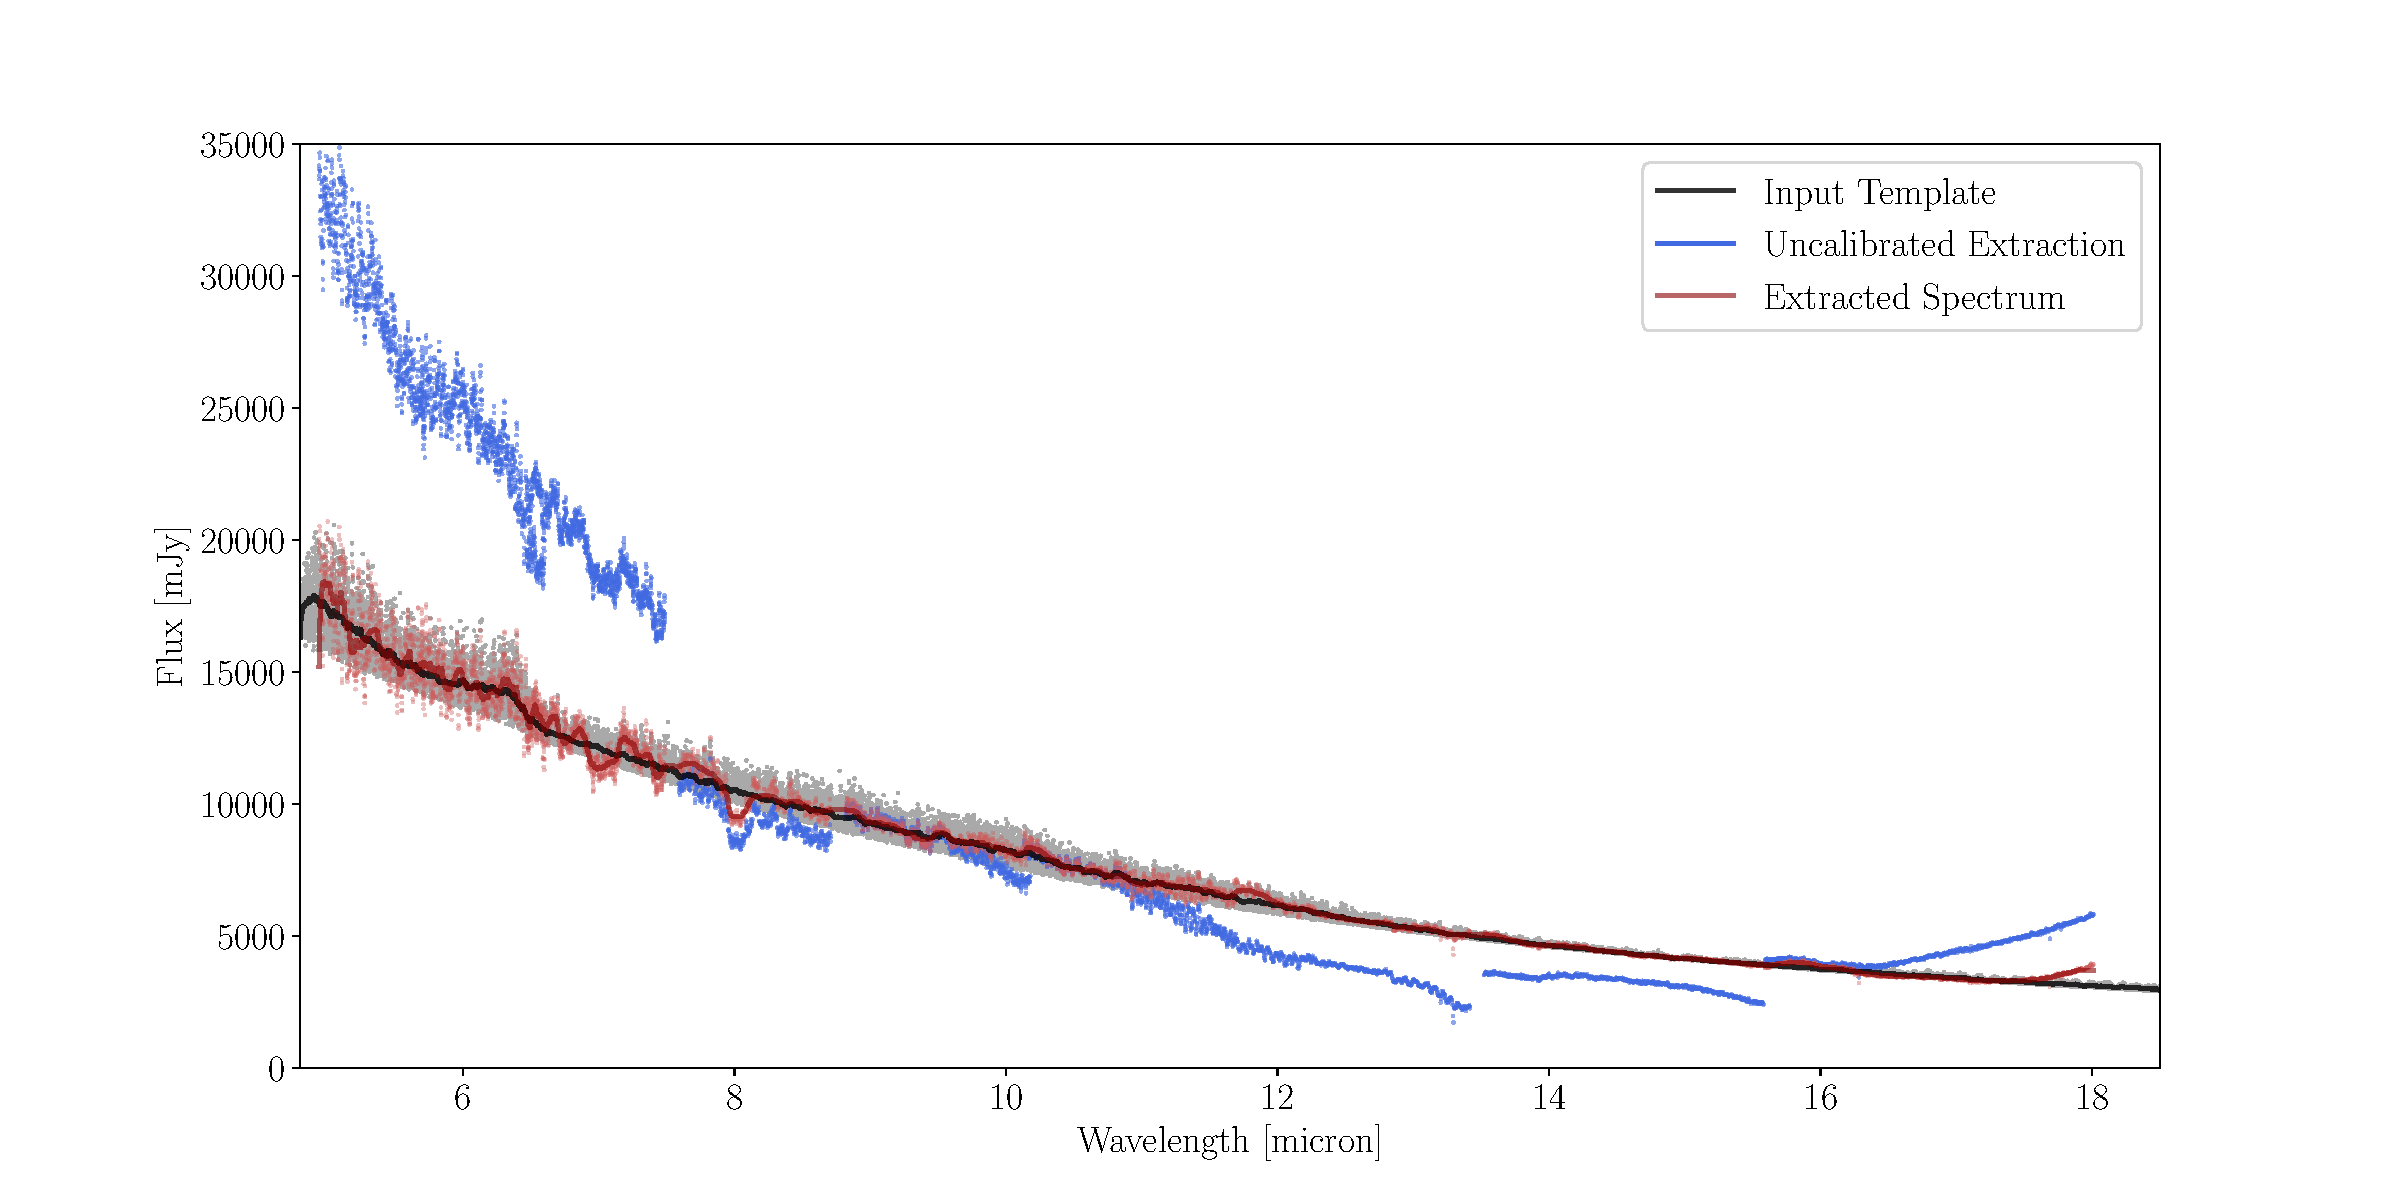
\includegraphics[width=1.11\linewidth]{cal_spectra_slope.pdf}
	\caption{Comparison of an input spectrum generated using petitRadTrans and the empirically calibrated output spectrum after extraction from the cube produced by the JWST pipeline.}
	\label{fig:cal}
\end{figure}

\subsection{Cross-Correlation}
\cite{Snellen2014}% BetaPicFast Rotation - cross correlation
\cite{Simkin1974} %Cross cor
\cite{Tonry1979} %Old cross corr
\cite{Petermann2019} %Robin thesis cross corr
\cite{Bodis2007} %Alternative to cc - spectral similarity
To quantify the similarity of the spectrum output by the JWST pipeline to the input into MIRISIM, we rely on the technique of cross correlation \cite{}.
For two arbitrary, complex-valued functions $f(t)$ and $g(t)$, we can compute the cross correlation as as function of the shift $\tau$ between the functions (typically in time or velocity space):
\begin{equation}\label{eqn:crosscorr}
\left(f \star g\right)(\tau) \equiv \int_{-\infty}^{\infty}f^{*}(t)g(t + \tau)dt
\end{equation}
Our signals of interest are astrophysical spectra, measured in a finite number of discrete wavelength bins. For such a signal with $M$ bins:
\begin{equation}\label{eqn:discretecorr}
\left(f \star g\right)[n] \equiv \sum_{m=0}^{M}f^{*}[m]g[m + n]
\end{equation}

Care must be taken when cross-correlating signals, as differences in normalization can result in changes in the correlation coefficient. 
Our procedure takes in two spectra. 
The first is an emission spectrum produced by the petitRadTrans program \cite{Molliere2019}, which provides our forward model with which we compare our data spectrum.
Our data is the result of passing the template spectrum through MIRISIM, and extracting it from the resulting detector image using the JWST pipeline.
We then rebin the high-resolution input spectrum to the same wavelength bins as the data spectrum, using the \verb|spectres| package \cite{}.
Prior to normalization, we remove any outliers from the spectrum (due to binning errors or instrumental effects) by setting any data points separater by more than 15 standard deviations from the mean to the median value of the spectrum.
For each spectrum, we subtract the minimum value to remove any offset in the spectrum, and divide by the maximum value to restrict the range to [0,1]. 
We then use apply a Savitzky-Golay filter with a window of 1/4 the length of the spectrum and a polynomial order of 3, which we then subtract from the unfiltered spectrum. 
This removes the continuum emission from the spectrum, and centers it around 0.
We then renormalize the spectrum by dividing by the maximum absolute value such that the range is in [-1,1]. 
The cross correlation between the forward model and itself is computed, excluding the region of interest around 0 offset. 
This `autocorrelation' is subtracted from the cross correlation between the forward model and the data spectrum in order to remove secondary peaks.
Finally, we normalize the cross correlation by the standard deviation of the cross correlation (excluding the central peak), giving an output measured as a signal to noise ratio.

\subsection{Residual Statistics}
In addition to computing the cross correlation between the forward model and the data spectrum, we also examine the residuals between the two spectra.
Here we can see any unexpected variations between the two (periodic signals, offsets or other features).
We can also examine a histogram of the residuals, normalized by the standard deviation of the data spectrum.
This provides us with a  distribution which should have a mean of 0 and unit width if the data are unbiased and share a distribution with the true input spectrum.
\section{Fringing Results}
1. A stronger input signal results in a stronger correlation.
2. Fringing does NOT necessarily degrade the cross correlation SNR, but rather increases it. The scale of this increase seems to depend on the absolute magnitude of the correlation (ie, a larger increase at higher SNR)
3. The residuals from subtracting the template from the data has structure.
4. If the residuals are histogrammed (and normalized by the standard deviation of the data), the width of the distribution may correspond to the cross correlation SNR (wider distribution = lower SNR)
5. Only when strongly increasing the fringing effect does the SNR decrease.
6. Correcting for fringing using the standard JWST fringe map decreases the SNR when compared to the case of fringing with no correction, but is typically still above the no-fringing case.
7. The JWST correction performs worse in the off axis case, as the fringe pattern begins to vary more when compared to the CV fringing model.
\subsection{Effects of fringing on spectral extraction}